% Options for packages loaded elsewhere
\PassOptionsToPackage{unicode}{hyperref}
\PassOptionsToPackage{hyphens}{url}
\PassOptionsToPackage{dvipsnames,svgnames,x11names}{xcolor}
%
\documentclass[
  letterpaper,
  DIV=11,
  numbers=noendperiod]{scrartcl}

\usepackage{amsmath,amssymb}
\usepackage{iftex}
\ifPDFTeX
  \usepackage[T1]{fontenc}
  \usepackage[utf8]{inputenc}
  \usepackage{textcomp} % provide euro and other symbols
\else % if luatex or xetex
  \usepackage{unicode-math}
  \defaultfontfeatures{Scale=MatchLowercase}
  \defaultfontfeatures[\rmfamily]{Ligatures=TeX,Scale=1}
\fi
\usepackage{lmodern}
\ifPDFTeX\else  
    % xetex/luatex font selection
\fi
% Use upquote if available, for straight quotes in verbatim environments
\IfFileExists{upquote.sty}{\usepackage{upquote}}{}
\IfFileExists{microtype.sty}{% use microtype if available
  \usepackage[]{microtype}
  \UseMicrotypeSet[protrusion]{basicmath} % disable protrusion for tt fonts
}{}
\makeatletter
\@ifundefined{KOMAClassName}{% if non-KOMA class
  \IfFileExists{parskip.sty}{%
    \usepackage{parskip}
  }{% else
    \setlength{\parindent}{0pt}
    \setlength{\parskip}{6pt plus 2pt minus 1pt}}
}{% if KOMA class
  \KOMAoptions{parskip=half}}
\makeatother
\usepackage{xcolor}
\setlength{\emergencystretch}{3em} % prevent overfull lines
\setcounter{secnumdepth}{5}
% Make \paragraph and \subparagraph free-standing
\makeatletter
\ifx\paragraph\undefined\else
  \let\oldparagraph\paragraph
  \renewcommand{\paragraph}{
    \@ifstar
      \xxxParagraphStar
      \xxxParagraphNoStar
  }
  \newcommand{\xxxParagraphStar}[1]{\oldparagraph*{#1}\mbox{}}
  \newcommand{\xxxParagraphNoStar}[1]{\oldparagraph{#1}\mbox{}}
\fi
\ifx\subparagraph\undefined\else
  \let\oldsubparagraph\subparagraph
  \renewcommand{\subparagraph}{
    \@ifstar
      \xxxSubParagraphStar
      \xxxSubParagraphNoStar
  }
  \newcommand{\xxxSubParagraphStar}[1]{\oldsubparagraph*{#1}\mbox{}}
  \newcommand{\xxxSubParagraphNoStar}[1]{\oldsubparagraph{#1}\mbox{}}
\fi
\makeatother

\usepackage{color}
\usepackage{fancyvrb}
\newcommand{\VerbBar}{|}
\newcommand{\VERB}{\Verb[commandchars=\\\{\}]}
\DefineVerbatimEnvironment{Highlighting}{Verbatim}{commandchars=\\\{\}}
% Add ',fontsize=\small' for more characters per line
\usepackage{framed}
\definecolor{shadecolor}{RGB}{241,243,245}
\newenvironment{Shaded}{\begin{snugshade}}{\end{snugshade}}
\newcommand{\AlertTok}[1]{\textcolor[rgb]{0.68,0.00,0.00}{#1}}
\newcommand{\AnnotationTok}[1]{\textcolor[rgb]{0.37,0.37,0.37}{#1}}
\newcommand{\AttributeTok}[1]{\textcolor[rgb]{0.40,0.45,0.13}{#1}}
\newcommand{\BaseNTok}[1]{\textcolor[rgb]{0.68,0.00,0.00}{#1}}
\newcommand{\BuiltInTok}[1]{\textcolor[rgb]{0.00,0.23,0.31}{#1}}
\newcommand{\CharTok}[1]{\textcolor[rgb]{0.13,0.47,0.30}{#1}}
\newcommand{\CommentTok}[1]{\textcolor[rgb]{0.37,0.37,0.37}{#1}}
\newcommand{\CommentVarTok}[1]{\textcolor[rgb]{0.37,0.37,0.37}{\textit{#1}}}
\newcommand{\ConstantTok}[1]{\textcolor[rgb]{0.56,0.35,0.01}{#1}}
\newcommand{\ControlFlowTok}[1]{\textcolor[rgb]{0.00,0.23,0.31}{\textbf{#1}}}
\newcommand{\DataTypeTok}[1]{\textcolor[rgb]{0.68,0.00,0.00}{#1}}
\newcommand{\DecValTok}[1]{\textcolor[rgb]{0.68,0.00,0.00}{#1}}
\newcommand{\DocumentationTok}[1]{\textcolor[rgb]{0.37,0.37,0.37}{\textit{#1}}}
\newcommand{\ErrorTok}[1]{\textcolor[rgb]{0.68,0.00,0.00}{#1}}
\newcommand{\ExtensionTok}[1]{\textcolor[rgb]{0.00,0.23,0.31}{#1}}
\newcommand{\FloatTok}[1]{\textcolor[rgb]{0.68,0.00,0.00}{#1}}
\newcommand{\FunctionTok}[1]{\textcolor[rgb]{0.28,0.35,0.67}{#1}}
\newcommand{\ImportTok}[1]{\textcolor[rgb]{0.00,0.46,0.62}{#1}}
\newcommand{\InformationTok}[1]{\textcolor[rgb]{0.37,0.37,0.37}{#1}}
\newcommand{\KeywordTok}[1]{\textcolor[rgb]{0.00,0.23,0.31}{\textbf{#1}}}
\newcommand{\NormalTok}[1]{\textcolor[rgb]{0.00,0.23,0.31}{#1}}
\newcommand{\OperatorTok}[1]{\textcolor[rgb]{0.37,0.37,0.37}{#1}}
\newcommand{\OtherTok}[1]{\textcolor[rgb]{0.00,0.23,0.31}{#1}}
\newcommand{\PreprocessorTok}[1]{\textcolor[rgb]{0.68,0.00,0.00}{#1}}
\newcommand{\RegionMarkerTok}[1]{\textcolor[rgb]{0.00,0.23,0.31}{#1}}
\newcommand{\SpecialCharTok}[1]{\textcolor[rgb]{0.37,0.37,0.37}{#1}}
\newcommand{\SpecialStringTok}[1]{\textcolor[rgb]{0.13,0.47,0.30}{#1}}
\newcommand{\StringTok}[1]{\textcolor[rgb]{0.13,0.47,0.30}{#1}}
\newcommand{\VariableTok}[1]{\textcolor[rgb]{0.07,0.07,0.07}{#1}}
\newcommand{\VerbatimStringTok}[1]{\textcolor[rgb]{0.13,0.47,0.30}{#1}}
\newcommand{\WarningTok}[1]{\textcolor[rgb]{0.37,0.37,0.37}{\textit{#1}}}

\providecommand{\tightlist}{%
  \setlength{\itemsep}{0pt}\setlength{\parskip}{0pt}}\usepackage{longtable,booktabs,array}
\usepackage{calc} % for calculating minipage widths
% Correct order of tables after \paragraph or \subparagraph
\usepackage{etoolbox}
\makeatletter
\patchcmd\longtable{\par}{\if@noskipsec\mbox{}\fi\par}{}{}
\makeatother
% Allow footnotes in longtable head/foot
\IfFileExists{footnotehyper.sty}{\usepackage{footnotehyper}}{\usepackage{footnote}}
\makesavenoteenv{longtable}
\usepackage{graphicx}
\makeatletter
\def\maxwidth{\ifdim\Gin@nat@width>\linewidth\linewidth\else\Gin@nat@width\fi}
\def\maxheight{\ifdim\Gin@nat@height>\textheight\textheight\else\Gin@nat@height\fi}
\makeatother
% Scale images if necessary, so that they will not overflow the page
% margins by default, and it is still possible to overwrite the defaults
% using explicit options in \includegraphics[width, height, ...]{}
\setkeys{Gin}{width=\maxwidth,height=\maxheight,keepaspectratio}
% Set default figure placement to htbp
\makeatletter
\def\fps@figure{htbp}
\makeatother
% definitions for citeproc citations
\NewDocumentCommand\citeproctext{}{}
\NewDocumentCommand\citeproc{mm}{%
  \begingroup\def\citeproctext{#2}\cite{#1}\endgroup}
\makeatletter
 % allow citations to break across lines
 \let\@cite@ofmt\@firstofone
 % avoid brackets around text for \cite:
 \def\@biblabel#1{}
 \def\@cite#1#2{{#1\if@tempswa , #2\fi}}
\makeatother
\newlength{\cslhangindent}
\setlength{\cslhangindent}{1.5em}
\newlength{\csllabelwidth}
\setlength{\csllabelwidth}{3em}
\newenvironment{CSLReferences}[2] % #1 hanging-indent, #2 entry-spacing
 {\begin{list}{}{%
  \setlength{\itemindent}{0pt}
  \setlength{\leftmargin}{0pt}
  \setlength{\parsep}{0pt}
  % turn on hanging indent if param 1 is 1
  \ifodd #1
   \setlength{\leftmargin}{\cslhangindent}
   \setlength{\itemindent}{-1\cslhangindent}
  \fi
  % set entry spacing
  \setlength{\itemsep}{#2\baselineskip}}}
 {\end{list}}
\usepackage{calc}
\newcommand{\CSLBlock}[1]{\hfill\break\parbox[t]{\linewidth}{\strut\ignorespaces#1\strut}}
\newcommand{\CSLLeftMargin}[1]{\parbox[t]{\csllabelwidth}{\strut#1\strut}}
\newcommand{\CSLRightInline}[1]{\parbox[t]{\linewidth - \csllabelwidth}{\strut#1\strut}}
\newcommand{\CSLIndent}[1]{\hspace{\cslhangindent}#1}

\KOMAoption{captions}{tableheading}
\makeatletter
\@ifpackageloaded{caption}{}{\usepackage{caption}}
\AtBeginDocument{%
\ifdefined\contentsname
  \renewcommand*\contentsname{Table of contents}
\else
  \newcommand\contentsname{Table of contents}
\fi
\ifdefined\listfigurename
  \renewcommand*\listfigurename{List of Figures}
\else
  \newcommand\listfigurename{List of Figures}
\fi
\ifdefined\listtablename
  \renewcommand*\listtablename{List of Tables}
\else
  \newcommand\listtablename{List of Tables}
\fi
\ifdefined\figurename
  \renewcommand*\figurename{Figure}
\else
  \newcommand\figurename{Figure}
\fi
\ifdefined\tablename
  \renewcommand*\tablename{Table}
\else
  \newcommand\tablename{Table}
\fi
}
\@ifpackageloaded{float}{}{\usepackage{float}}
\floatstyle{ruled}
\@ifundefined{c@chapter}{\newfloat{codelisting}{h}{lop}}{\newfloat{codelisting}{h}{lop}[chapter]}
\floatname{codelisting}{Listing}
\newcommand*\listoflistings{\listof{codelisting}{List of Listings}}
\makeatother
\makeatletter
\makeatother
\makeatletter
\@ifpackageloaded{caption}{}{\usepackage{caption}}
\@ifpackageloaded{subcaption}{}{\usepackage{subcaption}}
\makeatother

\ifLuaTeX
  \usepackage{selnolig}  % disable illegal ligatures
\fi
\usepackage{bookmark}

\IfFileExists{xurl.sty}{\usepackage{xurl}}{} % add URL line breaks if available
\urlstyle{same} % disable monospaced font for URLs
\hypersetup{
  pdftitle={A tutorial on Generalised Additive Mixed Effects Models for bilingualism research},
  colorlinks=true,
  linkcolor={blue},
  filecolor={Maroon},
  citecolor={Blue},
  urlcolor={Blue},
  pdfcreator={LaTeX via pandoc}}


\title{A tutorial on Generalised Additive Mixed Effects Models for
bilingualism research}
\author{}
\date{}

\begin{document}
\maketitle


Stefano Coretta (Linguistics and English Language, University of
Edinburgh, UK)

Joseph V. Casillas (Department of Spanish and Portuguese, Rutgers
University, USA)

\textbf{ABSTRACT}

While recent years have seen a shift towards random effects modelling,
particularly in areas of linguistics in which nested structure is the
norm (e.g., trial repetitions nested within participants), an
over-reliance on standard linear modelling prevails, particularly in the
cases of dynamic phenomena that may not constitute a linear
relationship, e.g., vowel trajectories, pitch contours, acquisition
processes, etc. Generalised Additive (Mixed) Models (GAMMs) are now
commonly employed in phonetic research (given the naturally dynamic
nature of speech data) and this is reflected by the availability of
several tutorials which focus on phonetic data. This tutorial aims at
making GAMMs accessible to researchers from other fields within
linguistics. In particular, this tutorial is written for researchers in
bilingualism and multilingualism who wish to be able to start using
GAMMs for non-linear data, which is very common in developmental and
learning phenomena. While only the basics will be covered here, we hope
that researchers will get the necessary foundations to be able to learn
GAMMs from existing resources.

\textbf{Keywords}: generalised additive mixed models; GAMMs; non-linear
data; dynamic analysis.

\section{Motivation}\label{motivation}

In recent years quantitative analysis of linguistic data has benefited
greatly from the now commonplace use of so-called random effects (also
known as hierarchical, mixed-effects, multi-level or nested models,
Winter (2013); Winter (2020)). While this shift represents a clear
improvement in statistical analyses, particularly in areas of
linguistics in which nested structure is the norm (e.g., trial
repetitions nested within participants), an over-reliance on standard
linear modelling prevails, particularly in the cases of dynamic
phenomena that may not constitute a linear relationship, e.g., vowel
trajectories, pitch contours, acquisition processes, etc.

Generalised Additive (Mixed) Models (GAMMs) are now commonly employed in
phonetic research (given the naturally dynamic nature of speech data)
and this is reflected by the availability of several tutorials which
focus on phonetic data (Sóskuthy, 2017, 2021; Tamminga et al., 2016;
Wieling, 2018), and biological data (Pedersen et al., 2019). We hope
that this tutorial will make GAMMs accessible to researchers from other
fields within linguistics as well. In particular, this tutorial has in
mind researchers focusing on bi- and multilingualism who wish to start
using GAMMs for non-linear data, which is common in developmental and
learning phenomena.

\subsection{Generalised additive (mixed)
models}\label{generalised-additive-mixed-models}

Generalised Additive Models (GAMs) and their mixed-effects version
(GAMMs) represent a variation of the generalised linear model that can
accommodate modelling non-linear relationships (Hastie \& Tibshirani,
1986; Wood, 2006). The main component specific to GAMMs is known as a
smoother or smooth term. These are model terms that can fit non-linear
effects. An advantage of using smooth terms is that they are constrained
by a smoothing penalty parameter. Importantly, this penalty parameter is
a standard part of the fitting procedure that does not depend on user
input and can help prevent over-fitting the data. This approach is
different from, for example, growth curve analyses which are based on
user-specified polynomial degrees. Note, however, that
under/over-fitting is still possible depending on the number of basis
functions used in building the smoothers (for a more detailed
explanation of basis functions, see the aforementioned tutorials).

The rest of this tutorial focuses on applying GAMMs in bilingualism
research using the statistical programming language R (R Core Team,
2023). While completing this tutorial will allow you to jump-start into
fitting basic GAMMs with the mgcv package Wood (2011), we invite
interested readers to peruse the tutorials mentioned above to avoid
unnecessary repetition of content here. Readers interested in a more
detailed conceptual discussion of GAMMs are referred to Sóskuthy (2017).
Finally, we opted not to treat statistical significance testing in GAMMs
(significance testing is treated in details in the aforementioned
tutorials).

\section{Pre-requisites}\label{pre-requisites}

In what follows, we detail the packages needed to complete the tutorial,
followed by two specific case studies designed to illustrate how GAMMs
can be applied to model common phenomena in second language acquisition
and bilingualism research.

This tutorial assumes readers are already familiar with R (R Core Team,
2023) and have at least some experience fitting linear models, including
models with random effects. The following packages need to be installed:

\begin{itemize}
\item
  tidyverse
\item
  mgcv
\item
  tidygam
\end{itemize}

All the tutorial code and data are freely available here:
\url{https://github.com/stefanocoretta/gamm_biling}.

\section{Case study 1: U-shaped
learning}\label{case-study-1-u-shaped-learning}

\subsection{U-shaped learning}\label{u-shaped-learning}

Research on language acquisition first documented over-regularization
errors in the 60's (Cazden, 1968; Ervin \& Miller, 1963). Subsequent
research found that over-regularization errors tended to manifest in a
developmental curve, and is now referred to as the \emph{U-shaped
developmental curve} (Botezatu et al., 2024; Williams et al., 2022). In
most cases, U-shaped development is considered to be a three-step
process, which begins with accurate performance, followed by a period in
which performance dips, and then subsequently becomes accurate again
(Carlucci \& Case, 2013). Interestingly, U-shaped curves are observed in
numerous cognitive-developmental and learning contexts, particularly
with regard to child development, e.g., understanding temperature,
weight conservation, object permanence, and facial recognition (See
Carlucci \& Case, 2013), which, in turn, has fostered fruitful research
and debate in Cognitive Science regarding learning models (e.g., Marcus
et al., 1992; Rumelhart \& McClelland, 1986, among others).

In first language acquisition research, the most cited example stems
from children's use of the past tense (Cazden, 1968; Ervin \& Miller,
1963; Marcus et al., 1992). For instance, Cazden (1968) found that
children accurately produced irregular past tense verbs during a period
of time, and, at a later point in time, began to produce
over-generalization errors, e.g., \emph{feet} followed by *\emph{feets}.
Eventually past tense production again surfaces as expected, typically
around the age of three, which coincides with the developmental stage in
which children acquire regular past tense verbs (See Marcus et al.,
1992). In the realm of Second Language Acquisition (SLA), researchers
have documented non-linear, U-shaped courses of development in numerous
areas for both developmental and instructional sequences (See Casani,
2020; Geeslin \& Guijarro-Fuentes, 2006; Kellerman, 1985; Long, 1990;
Pliatsikas \& Marinis, 2013; Shirai, 1990; Williams et al., 2022, among
many others). Kellerman (1985), for instance, documented Dutch learners
of English acquiring verb alternation patterns of English following a
U-shaped trajectory. In a similar vein, Lightbown (1983) showed accuracy
producing progressive forms (i.e., \emph{-ing}) followed a U-shaped
trajectory when acquiring the simple present/present continuous
tense/aspect distinction in French speaking learners of English.
U-shaped learning may be a by-product of reorganization or restructuring
of prior knowledge (Gass \& Selinker, 2008; Shirai, 1990), and likely
accounts for language instructors' contention that students often
regress when learning new linguistic forms. Be that as it may, it is
clear that the non-linear quality of this aspect of language learning
requires a non-linear approach to modelling the underlying process.

\subsection{The data}\label{the-data}

We have simulated data for accuracy scores from 200 language learners,
taken at 10 different time points. Note that the simulated data follow a
Gaussian (normal) distribution for pedagogical reasons, as it is a
straightforward distribution to use when introducing readers to new
statistical models. That being said, it is important to recognize that
real learner's data `in the wild' is seldom Gaussian. A proficiency
score was also included for each participant at each time point. The
data is intended to simulate a study in which participants perform the
same learning task and proficiency assessment in a longitudinal design.
We print the first six rows of the data frame below. Note that text
following a \textbackslash\# symbol is a comment and intended to aid the
reader in understanding the code.

\begin{Shaded}
\begin{Highlighting}[]
\CommentTok{\# Load data into R}
\NormalTok{dat1 }\OtherTok{\textless{}{-}} \FunctionTok{readRDS}\NormalTok{(}\StringTok{"data/dat1.rds"}\NormalTok{)}

\CommentTok{\# Print first 6 rows of the dataframe}
\FunctionTok{head}\NormalTok{(dat1)}
\end{Highlighting}
\end{Shaded}

\begin{verbatim}
# A tibble: 6 x 4
  score proficiency subj   time
  <dbl>       <dbl> <fct> <int>
1  26.7      -1.37  s1        0
2  26.4      -1.29  s1        1
3  26.0      -1.21  s1        2
4  25.7      -1.14  s1        3
5  25.5      -1.06  s1        4
6  25.2      -0.983 s1        5
\end{verbatim}

The \texttt{score} column contains the accuracy scores, while the
\texttt{proficiency} column the proficiency scores. The participant ID
is given in \texttt{subj}. The time point, 0 to 9, is in the
\texttt{time} column. Figure~\ref{fig-dat1} shows the relationship
between proficiency and learning scores for individual participants.
From the figure, it is clear that such relationship has a non-linear,
U-shape, in which learning scores initially decrease, plateau, then
increase again as proficiency increases.

\begin{figure}

\centering{

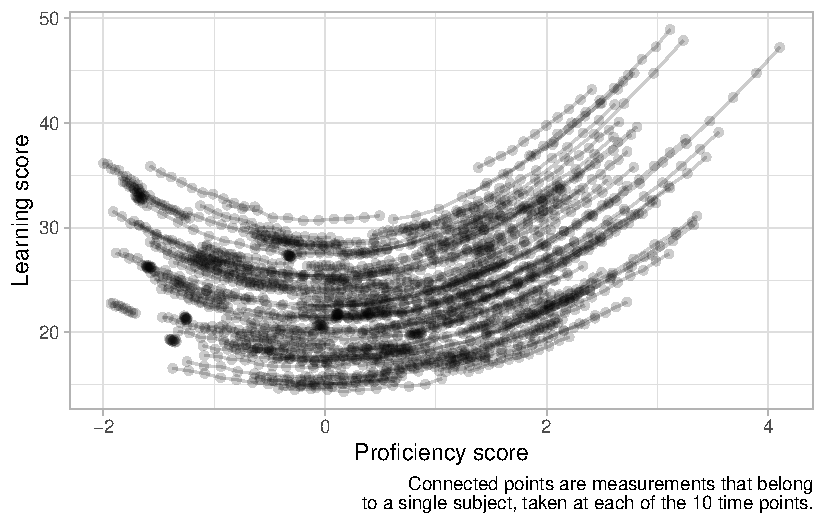
\includegraphics{manuscript_files/figure-pdf/fig-dat1-1.pdf}

}

\caption{\label{fig-dat1}Scatter plot of proficiency and learning scores
illustrating a U-shaped learning curve.}

\end{figure}%

In the following sections we will analyse this data using GAMMs. For
pedagogical purposes, we will first focus on the effect of proficiency
scores on learning scores at a single time point, time point 5.
Subsequently, we will analyse the entire data set to illustrate how to
conduct a time-series analysis.

\subsection{Modelling a non-linear
effect}\label{modelling-a-non-linear-effect}

Let's first focus on how to model a non-linear effect: here, we can look
at the effect of the proficiency score on learner accuracy. As we have
seen in Figure~\ref{fig-dat1}, the effect is U-shaped, i.e.~it is not
linear. To simplify, we will begin our analysis using data from a single
time point. Later we will expand the analysis to also include time as a
predictor. We model a non-linear effect of proficiency on accuracy with
the following code.

\begin{Shaded}
\begin{Highlighting}[]
\CommentTok{\# Subset the data to include only time point 5, assign subset to \textquotesingle{}dat15\textquotesingle{}}
\NormalTok{dat15 }\OtherTok{\textless{}{-}} \FunctionTok{filter}\NormalTok{(dat1, time }\SpecialCharTok{==} \DecValTok{5}\NormalTok{)}

\CommentTok{\# Load the mgcv package}
\FunctionTok{library}\NormalTok{(mgcv)}

\CommentTok{\# Fit the model, assign the model object to \textquotesingle{}gam\_1\textquotesingle{}}
\NormalTok{gam\_1 }\OtherTok{\textless{}{-}} \FunctionTok{gam}\NormalTok{(}
  \AttributeTok{formula =}\NormalTok{ score }\SpecialCharTok{\textasciitilde{}} \FunctionTok{s}\NormalTok{(proficiency),}
  \AttributeTok{data =}\NormalTok{ dat15}
\NormalTok{)}
\end{Highlighting}
\end{Shaded}

The formula states that \texttt{score}, the outcome variable (also known
as the dependent variable or criterion) is modelled as a function of
\texttt{proficiency}. Note that we use \texttt{s()} to indicate that we
want to estimate a (potentially) non-linear effect of proficiency. The
name of the function, \texttt{s}, stands for ``smooth term''. Smooth
terms (aka smoothers) are mathematical functions that allow GAMs to fit
non-linear effects. A detailed treatment of smoothers is beyond the
scope of this tutorial. We refer readers to Wood (2006) for a
mathematical description and to other existing tutorials for a gentler
introduction (Pedersen et al., 2019; e.g., Sóskuthy, 2017; Wieling,
2018).

Before looking at the summary of the \texttt{gam\_1} model, we plot the
predicted effect of proficiency. For this, we will use the
\texttt{tidygam} package (Coretta, 2023), which provides users with
utility functions that make extracting and plotting predictions from
GAMs more accessible.

\begin{Shaded}
\begin{Highlighting}[]
\CommentTok{\# Load tidygam package}
\FunctionTok{library}\NormalTok{(tidygam)}

\CommentTok{\# Extract model predictions from \textquotesingle{}gam\_1\textquotesingle{}, assign them to \textquotesingle{}gam\_1\_preds\textquotesingle{}}
\NormalTok{gam\_1\_preds }\OtherTok{\textless{}{-}} \FunctionTok{predict\_gam}\NormalTok{(gam\_1)}

\CommentTok{\# Plot predictions}
\FunctionTok{plot}\NormalTok{(gam\_1\_preds, }\AttributeTok{series =} \StringTok{"proficiency"}\NormalTok{)}
\end{Highlighting}
\end{Shaded}

\begin{figure}[H]

\centering{

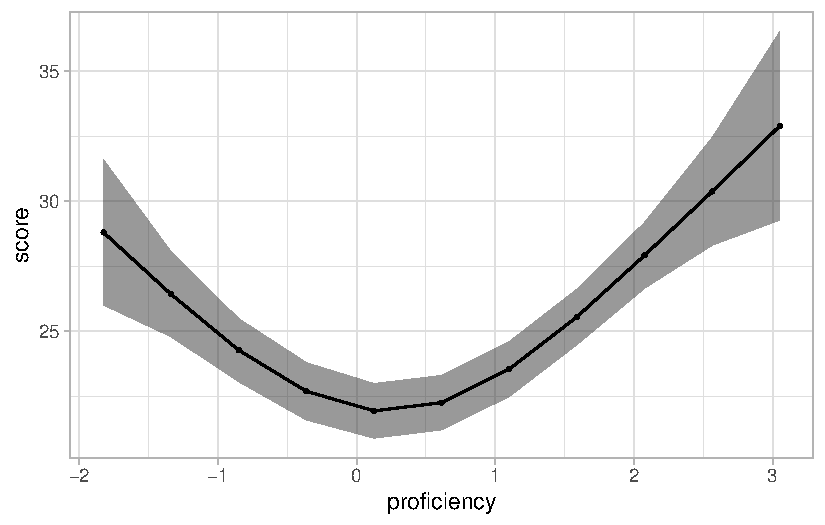
\includegraphics{manuscript_files/figure-pdf/fig-gam-1-1.pdf}

}

\caption{\label{fig-gam-1}Predicted accuracy score depending on
proficiency, from a GAM.}

\end{figure}%

Figure~\ref{fig-gam-1} is a plot of the predicted effect of proficiency
on accuracy, based on the \texttt{gam\_1} model. We will look into the
details of \texttt{predict\_gam()} shortly, but for now, notice that
accuracy initially decreases as proficiency increases. At a proficiency
score of approximately 0.5, accuracy begins to increase, resulting in
the typical U-shaped curve described above. At this juncture we will
inspect the model summary.

\begin{Shaded}
\begin{Highlighting}[]
\CommentTok{\# Print a summary of the model \textquotesingle{}gam\_1\textquotesingle{}}
\FunctionTok{summary}\NormalTok{(gam\_1)}
\end{Highlighting}
\end{Shaded}

\begin{verbatim}

Family: gaussian 
Link function: identity 

Formula:
score ~ s(proficiency)

Parametric coefficients:
            Estimate Std. Error t value Pr(>|t|)    
(Intercept)   24.559      0.331   74.19   <2e-16 ***
---
Signif. codes:  0 '***' 0.001 '**' 0.01 '*' 0.05 '.' 0.1 ' ' 1

Approximate significance of smooth terms:
                 edf Ref.df     F p-value    
s(proficiency) 2.922  3.675 16.46  <2e-16 ***
---
Signif. codes:  0 '***' 0.001 '**' 0.01 '*' 0.05 '.' 0.1 ' ' 1

R-sq.(adj) =  0.242   Deviance explained = 25.3%
GCV = 22.352  Scale est. = 21.914    n = 200
\end{verbatim}

The relevant parts of the summary for the time being are the
\texttt{Parametric\ coefficients:} table and the
\texttt{Approximate\ significance\ of\ smooth\ terms:} table. The former
contains the estimate of the intercept. This intercept represents the
same intercept you would estimate in a standard linear model. In our
case, the estimate of the intercept is the predicted accuracy score when
proficiency is equal to zero. Thus our interpretation according to the
summary, is that when proficiency is 0, learner accuracy is about 25.

Importantly, what we are interested in is the effect of proficiency on
accuracy, rather than the estimate of accuracy when proficiency is zero,
i.e., the intercept. Information on the effect of proficiency is found
in the second table, which contains estimates of the smooth terms. Alas,
these estimates are not informative about the effect, per se, but rather
indicate if the relationship between proficiency and accuracy is linear
(or not) in nature. More specifically, the \texttt{edf} estimate, which
stands for Estimated Degrees of Freedom, is equal to one in the case of
a perfectly linear relationship. A value greater than one is an
indication of non-linear effects. Crucially, the EDF estimate is not
informative with regard to the exact shape of the effect. The only way
to assess this is to plot the model predictions, as we have done in
Figure~\ref{fig-gam-1}.

In our \texttt{gam\_1} model, the \texttt{edf} of the smooth term for
proficiency is 2.9, thus suggesting that the effect of proficiency on
accuracy is not linear (Note: the \texttt{Ref.df}, reference degrees of
freedom, and \texttt{F} values merely serve the purpose of being used to
derive a \emph{p}-value). The \emph{p}-value indicates the probability
of the observed smooth under the null hypothesis that the smooth is a
horizontal flat line (in other words, under the null hypothesis that the
variable of the smooth has no effect on the outcome variable, Simpson
(2023)).

If we were to report this model and interpret the results, we could
write something along the following lines: We fitted a Generalised
Additive Model to learner accuracy scores, with a smooth term over
proficiency (to model non-linear effects). According to the model, the
effect of proficiency is non-linear and significant (\emph{F} = 16.46,
\emph{p} \textless{} 0.0001). Based on the prediction plot, we observe
that at lower proficiency, learning scores initially decrease and then
start increasing again when proficiency reaches approximately 0.5.

We began our analysis with a simplified model examining the effect of
proficiency on accuracy at a single time point for pedagogical purposes.
In the following section we will expand our analysis by refitting the
data including time as a predictor.

\subsection{Multiple smooth terms}\label{multiple-smooth-terms}

As mentioned previously, the data \texttt{dat1} contains accuracy and
proficiency scores from 200 subjects, taken at 10 time points. The data
was simulated so that proficiency increased over time (at different
degrees for different participants), as is often the case in language
acquisition processes. An interesting question to consider is whether
learning scores improve with time independently of proficiency, or if
proficiency alone is causing learning scores to improve. We can approach
this question using principles of causal inference. To this end, we
develop directed acyclic graphs (DAGs) to describe the causal
relationships involved. Though a full treatment of causal inference is
beyond the scope of this paper, we believe the DAG is informative in
aiding understanding of the model we will build. Readers interested in a
deep dive into causal inference and DAGs are referred to McElreath
(2019) and Pearl (2010).

The DAGs in Figure~\ref{fig-d1-dag} represent the causal relationships
between accuracy, proficiency scores and time in two scenarios. In (a),
time affects proficiency and proficiency affects accuracy. In other
words, time has a direct effect on proficiency, but not on accuracy;
accuracy scores can be predicted from proficiency alone. In (b), on the
other hand, time affects proficiency, as in (a), but also accuracy (and
proficiency affects accuracy scores as in (a)). The practical
interpretation is that time affects accuracy in two ways: through its
effect on proficiency and directly through its effect on accuracy.

\begin{figure}

\begin{minipage}{0.50\linewidth}

\centering{

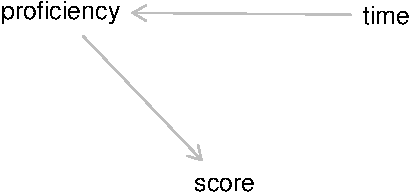
\includegraphics{manuscript_files/figure-pdf/fig-d1-dag-1.pdf}

}

\subcaption{\label{fig-d1-dag-1}No direct effect of time on learning
scores.}

\end{minipage}%
%
\begin{minipage}{0.50\linewidth}

\centering{

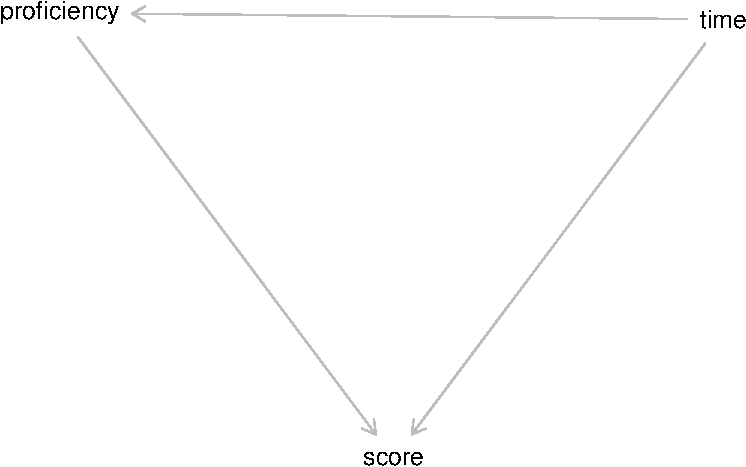
\includegraphics{manuscript_files/figure-pdf/fig-d1-dag-2.pdf}

}

\subcaption{\label{fig-d1-dag-2}Direct effect of time on learning
scores.}

\end{minipage}%

\caption{\label{fig-d1-dag}Directed Acyclic Graphs for time, proficiency
and learning score.}

\end{figure}%

DAGs allow us to make causal statements based on statistical results. In
this case, when including both time and proficiency as predictors in a
GAM, time should not have an effect on learner accuracy if scenario (a)
is correct (while it should have an effect if scenario (b) is correct).
Now we fit the model.

\begin{Shaded}
\begin{Highlighting}[]
\CommentTok{\# Fit model, assign to \textquotesingle{}gam\_2\textquotesingle{}}
\NormalTok{gam\_2 }\OtherTok{\textless{}{-}} \FunctionTok{gam}\NormalTok{(}
  \AttributeTok{formula =}\NormalTok{ score }\SpecialCharTok{\textasciitilde{}} \FunctionTok{s}\NormalTok{(proficiency) }\SpecialCharTok{+} \FunctionTok{s}\NormalTok{(time) }\SpecialCharTok{+} \FunctionTok{s}\NormalTok{(subj, }\AttributeTok{bs =} \StringTok{"re"}\NormalTok{),}
  \AttributeTok{data =}\NormalTok{ dat1}
\NormalTok{)}
\end{Highlighting}
\end{Shaded}

In \texttt{gam\_2} we fit a GAM to learner accuracy \texttt{score} with
two predictors: a smooth term over proficiency and a smooth term over
time. We also include random effects to account for nested data from
multiple participants. The syntax for random effects in GAMs is
different from the more familiar syntax used in lme4. With
\texttt{gam()}, we can specify random effects using smooth terms and the
argument \texttt{re} (for Random Effects) basis function. Random
intercepts are added with the syntax
\texttt{s(INTERCEPT\_EFFECT,\ bs\ =\ "re")} and random slopes with the
syntax \texttt{s(INTERCEPT\_EFFECT,\ SLOPE\_EFFECT,\ bs\ =\ "re")}. Here
we only include a by-subject random intercept for illustration, i.e.,
\texttt{s(subj,\ bs\ =\ "re")}. Below we inspect the model summary.

\begin{Shaded}
\begin{Highlighting}[]
\CommentTok{\# Print summary of model \textquotesingle{}gam\_2\textquotesingle{}}
\FunctionTok{summary}\NormalTok{(gam\_2)}
\end{Highlighting}
\end{Shaded}

\begin{verbatim}

Family: gaussian 
Link function: identity 

Formula:
score ~ s(proficiency) + s(time) + s(subj, bs = "re")

Parametric coefficients:
            Estimate Std. Error t value Pr(>|t|)    
(Intercept)   24.738      0.441   56.09   <2e-16 ***
---
Signif. codes:  0 '***' 0.001 '**' 0.01 '*' 0.05 '.' 0.1 ' ' 1

Approximate significance of smooth terms:
                   edf  Ref.df       F  p-value    
s(proficiency)   8.699   8.976 4638.38  < 2e-16 ***
s(time)          1.000   1.000   20.27 7.36e-06 ***
s(subj)        198.943 200.000 2637.63  < 2e-16 ***
---
Signif. codes:  0 '***' 0.001 '**' 0.01 '*' 0.05 '.' 0.1 ' ' 1

R-sq.(adj) =  0.997   Deviance explained = 99.7%
GCV = 0.10023  Scale est. = 0.090681  n = 2200
\end{verbatim}

Now we plot the model predictions of accuracy score by proficiency and
time point separately.

\begin{Shaded}
\begin{Highlighting}[]
\CommentTok{\# Get model predictions for \textquotesingle{}proficiency\textquotesingle{}, assign them to \textquotesingle{}gam\_2\_preds\textquotesingle{}}
\NormalTok{gam\_2\_preds }\OtherTok{\textless{}{-}} \FunctionTok{predict\_gam}\NormalTok{(}
\NormalTok{  gam\_2, }\AttributeTok{length\_out =} \DecValTok{25}\NormalTok{,}
  \AttributeTok{series =} \StringTok{"proficiency"}\NormalTok{,}
  \AttributeTok{exclude\_terms =} \FunctionTok{c}\NormalTok{(}\StringTok{"s(subj)"}\NormalTok{)}
\NormalTok{)}
\end{Highlighting}
\end{Shaded}

\begin{Shaded}
\begin{Highlighting}[]
\CommentTok{\# Plot predictions}
\FunctionTok{plot}\NormalTok{(gam\_2\_preds)}
\end{Highlighting}
\end{Shaded}

\begin{figure}[H]

\centering{

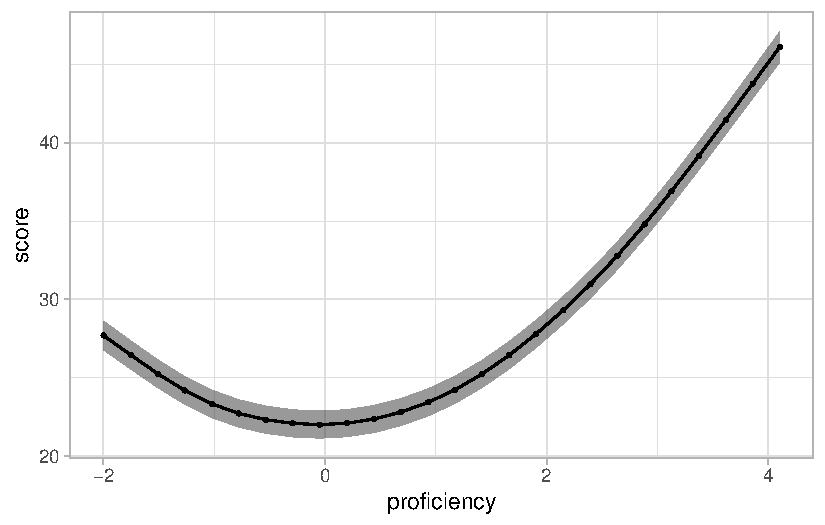
\includegraphics{manuscript_files/figure-pdf/fig-gam-2-preds-1.pdf}

}

\caption{\label{fig-gam-2-preds}Predicted accuracy score as a function
of proficiency, from a GAM.}

\end{figure}%

\begin{Shaded}
\begin{Highlighting}[]
\CommentTok{\# Get model predictions for \textquotesingle{}time\textquotesingle{}, assign them to \textquotesingle{}gam\_2\_preds\_t\textquotesingle{}}
\NormalTok{gam\_2\_preds\_t }\OtherTok{\textless{}{-}} \FunctionTok{predict\_gam}\NormalTok{(}
\NormalTok{  gam\_2, }\AttributeTok{length\_out =} \DecValTok{25}\NormalTok{,}
  \AttributeTok{series =} \StringTok{"time"}\NormalTok{,}
  \AttributeTok{exclude\_terms =} \FunctionTok{c}\NormalTok{(}\StringTok{"s(subj)"}\NormalTok{)}
\NormalTok{)}
\end{Highlighting}
\end{Shaded}

\begin{Shaded}
\begin{Highlighting}[]
\CommentTok{\# Plot predictions}
\FunctionTok{plot}\NormalTok{(gam\_2\_preds\_t) }\SpecialCharTok{+}
  \FunctionTok{ylim}\NormalTok{(}\DecValTok{20}\NormalTok{, }\DecValTok{45}\NormalTok{)}
\end{Highlighting}
\end{Shaded}

\begin{figure}[H]

\centering{

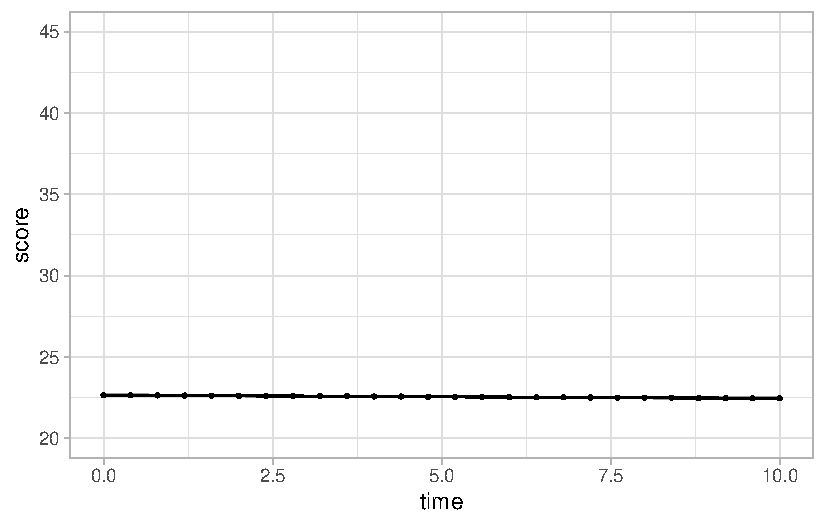
\includegraphics{manuscript_files/figure-pdf/fig-gam-2-preds-t-1.pdf}

}

\caption{\label{fig-gam-2-preds-t}Predicted accuracy score as a function
of time, from a GAM.}

\end{figure}%

Figure~\ref{fig-gam-2-preds} clearly shows a non-linear effect of
proficiency on accuracy scores. On the other hand,
Figure~\ref{fig-gam-2-preds-t} indicates that, once accounting for the
effect of proficiency, time has virtually no effect on accuracy, as
expected based on the data simulation and DAGs. Note that according to
the model the effect of time is linear but \emph{non-zero,} hence the
significant \emph{p-}value for that smooth. The effect is, nonetheless,
practically zero for two reasons: (1) first, the data was simulated in
such a way that time has no effect; (2) second, when inspecting the
predicted effect one can see that the mean difference in accuracy score
between time point 1 and 11 is about 0.2, which on the simulated
accuracy scale is negligible. This constitutes a nice caveat about
issues with significance testing (see Gigerenzer (2004) for more on the
topic). Generally, we advise researchers to rely more on model plotting
to assess effects.

We could report this model like so: We fitted a Generalised Additive
Model to learner accuracy scores, with a smooth term over proficiency
(to model non-linear effects of proficiency) and a smooth term over time
(to model non-linear effects of time). We also included a random
intercept smooth for subject (to account for overall difference in mean
accuracy by subject). According to the model, the effect of proficiency
is non-linear and significant (\emph{F} = 4638.38, \emph{p} \textless{}
0.0001). Based on the prediction plot, we observe that at lower
proficiency, learning scores initially decrease and then start
increasing again when proficiency reaches approximately 0.5. While the
model summary indicates a significant effect of time on accuracy, the
effect is negligibly small, which can be observed in the prediction plot
of time. To summarise, the model suggests a non-linear effect of
proficiency on learners' accuracy scores, but no effect of time.

In this example, we examined u-shaped development in second language
acquisition. Specifically, we explored a simulated data set and fit a
series of models, increasing in complexity. Our modelling strategy was
outlined \emph{a priori} using a DAG. We illustrated how to incorporate
non-linear effects into the model via smoothing terms using the function
\texttt{s()} inside the call to \texttt{gam()}. Next, we focused on
using the fitted object to generate and plot predictions using
\texttt{predict\_gam()} and, finally, we walked through how one can
report the resulting analysis. In the next section, we will consider
vowel production in bilingual speech.

\section{Case study 2: L2 vowel production in simultaneous and late
bilinguals}\label{case-study-2-l2-vowel-production-in-simultaneous-and-late-bilinguals}

To motivate our next example, we will now consider the production of
Spanish vowels in three groups of bilinguals: simultaneous/native
English/Spanish bilinguals (henceforth \texttt{es}) and late learners of
Spanish with low and high levels of proficiency, \texttt{es\_0} and
\texttt{es\_1}, respectively. Spanish has five phonemic vowels, /i, e,
a, o, u/, and is often described as being a syllable-timed language in
which the spectral envelope is rather stable and stressed and unstressed
syllables have approximately the same duration. Though there is evidence
that unstressed vowels can centralize to a certain degree, the
differences between stressed and unstressed vowels are believed to be
imperceptible (Martínez Celdrán, 1984). American English, on the other
hand, has a larger vowel inventory and is often described as a
stress-timed language in which the duration between stressed syllables
is approximately the same. Vowel reduction can occur in unstressed
syllables, which typically manifests via shortening and/or
centralization, with unstressed vowels often reducing to schwa
({[}ə{]}). Accordingly, English speaking learners of Spanish face a
substantial obstacle when it comes to producing and perceiving Spanish
vowels (See Aldrich, 2014; Bland, 2016; Cobb, 2009; Cobb \& Simonet,
2015; Iruela, 1997, among others). To wit, they often display
cross-linguistic influence by producing unstressed Spanish vowels with
{[}ə{]}, particularly in the case of /a/, e.g., ``casa'' (Eng.
\emph{house}) as {[}ka.sə{]}, and diphthongizing vowels in final
position (Cobb \& Simonet, 2015).

In the following example, we consider the production of Spanish vowels
in the aforementioned groups of bilingual participants. Interestingly,
to our knowledge, all of the current research investigating the
cross-linguistic influence of vowel reduction processes in learners of
Spanish have utilized modelling strategies that rely upon formant
measurements at a single time point, typically the mid-point of the
vowel, rather than scrutinizing the entire trajectory of the spectral
envelope (See de la Fuente Iglesias \& P'erez Castillejo (2022) and
Amengual \& Simonet (2020)). In our view, the dynamic nature of vowel
formants poses an interesting use-case for modelling using non-linear
methods, such as GAMs. To this end, we have simulated phonetic data from
three aforementioned groups of bilinguals: simultaneous English/Spanish
bilinguals, beginner late English/Spanish bilinguals and advanced late
English/Spanish bilinguals. The data contains the Euclidean Distance
(EuD) of three Spanish vowels /a, i, u/ from the vowel space centroid,
taken from word-final non-stressed vowels, along nine equidistant time
points. The measure is a good proxy for vowel reduction phenomena, which
is to be expected in late bilinguals.

\begin{Shaded}
\begin{Highlighting}[]
\CommentTok{\# Load data set}
\NormalTok{dat2 }\OtherTok{\textless{}{-}} \FunctionTok{readRDS}\NormalTok{(}\StringTok{"data/dat2.rds"}\NormalTok{)}

\CommentTok{\# Print first 6 rows}
\FunctionTok{head}\NormalTok{(dat2)}
\end{Highlighting}
\end{Shaded}

\begin{verbatim}
# A tibble: 6 x 7
  subj  group vowel   rep   eud timep id    
  <fct> <chr> <chr> <int> <dbl> <int> <chr> 
1 es_1  es    i         1  1.85     1 es.1.1
2 es_1  es    i         1  1.86     2 es.1.1
3 es_1  es    i         1  1.83     3 es.1.1
4 es_1  es    i         1  1.87     4 es.1.1
5 es_1  es    i         1  1.89     5 es.1.1
6 es_1  es    i         1  1.81     6 es.1.1
\end{verbatim}

The above code prints the first six rows of the data frame.
Specifically, we observe a subset of the synthetic data of a
simultaneous English/Spanish bilinguals (\texttt{es\_1}). It can be
observed in Figure~\ref{fig-dat2} that for the \texttt{es} group (top
row), the Euclidean distance is quite stable across the duration of the
vowel for all three vowels and away from 0 (which corresponds to a
mid-central vowel), indicating no reduction takes place (as is to be
expected for Spanish). On the other hand, in the second and third row of
Figure~\ref{fig-dat2}, we can see some vowel reduction at play: for /a/,
beginner late bilinguals (\texttt{es\_0}, middle row) completely reduce
the vowel to a mid-central vowel, while the advanced late bilinguals
(\texttt{es\_1}, bottom row) reduce to a lesser degree; /i/ and /u/ are
produced with a diphthongal quality, where the first part of the vowel
is quite reduced. In sum, comparing beginners and advanced bilinguals
shows that the latter have less reduction, presumably a by-product of
increasing proficiency in Spanish.

\begin{figure}

\centering{

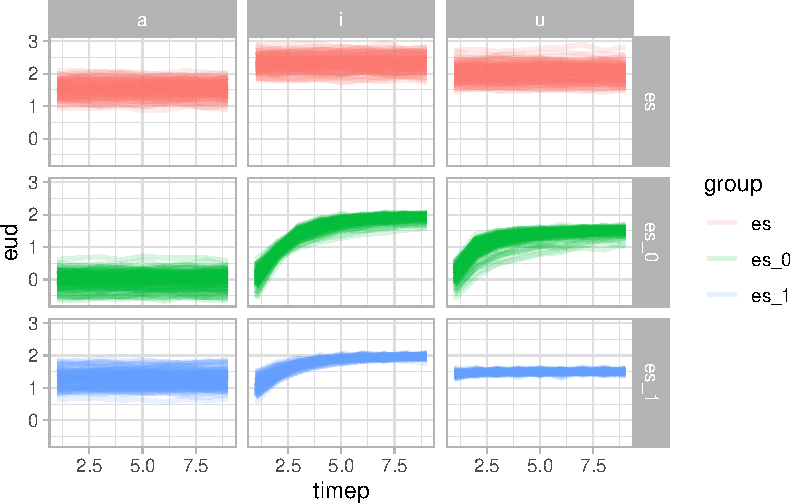
\includegraphics{manuscript_files/figure-pdf/fig-dat2-1.pdf}

}

\caption{\label{fig-dat2}Euclidean Distance through 9 time points taken
from within vowels.}

\end{figure}%

We can use a GAM to model the Euclidean distance along time points in
the different vowels and different bilingual groups. Fitting smooth
terms for different levels of categorical predictors can be achieved by
specifying the categorical predictor as the value of the \texttt{by}
argument inside the smooth term function \texttt{s()}. For example,
\texttt{s(timep,\ by\ =\ vowel)} would ensure a non-linear effect of
time point is estimated for each vowel. In our data, we want to model
the interaction of vowel (/a, i, u/) and group
(\texttt{es,\ es\_0,\ es\_1}). Unfortunately, the additive nature of
GAMs does not allow the direct specification of interactions between
smooth terms like one would do in a linear model (interactions require
product operations). Note that interactions between parametric terms are
supported, but these allow only for interactions in the overall height
of the smoothers, not in their shape. The method presented in this
section allows users to specify ``interactions'' in smooth terms that
can model differences in both height and shape.

To include interactions between smooth terms, we can simply construct a
new predictor with the combination of vowel and group and use that as
the \texttt{by}-variable in the smooth terms. Due to how smooth terms
are constructed when you include a \texttt{by}-variable, it is necessary
to also include the variable as a parametric term (i.e.~a classical
linear term). We would also like to allow for the modelled trajectories
to vary by subject both in height and shape. While random effects
included with \texttt{bs\ =\ "re"} (which we used in the first case
study) account for difference in height and rotation of the fitted
curves, \emph{random factor smooth interaction} terms fit a different
curve to each level of the chosen factor (in our case, subject). Random
factor smooth interaction terms are specified with \texttt{bs\ =\ "fs"}:
the first argument in \texttt{s()} should be the variable to smooth over
(here, \texttt{timep}) and the second argument is the factor (here
\texttt{subj}), the levels of which will be fitted separately. Finally,
the \texttt{m} argument corresponds to the order of the smoothing
penalty: higher orders lead to more smoothing (the default is
\texttt{2}, a second-order penalty). Setting \texttt{m\ =\ 1}
corresponds to a higher constraint on the smooths of each level in the
random factor, and it is thus a safeguard against over-fitting.

\begin{Shaded}
\begin{Highlighting}[]
\CommentTok{\# Generate group\_vowel column to model the interaction}
\NormalTok{dat2 }\OtherTok{\textless{}{-}}\NormalTok{ dat2 }\SpecialCharTok{|\textgreater{}}
  \FunctionTok{mutate}\NormalTok{(}
    \AttributeTok{vowel =} \FunctionTok{as.factor}\NormalTok{(vowel),}
    \AttributeTok{group\_vowel =} \FunctionTok{interaction}\NormalTok{(group, vowel),}
\NormalTok{  )}
\end{Highlighting}
\end{Shaded}

\begin{Shaded}
\begin{Highlighting}[]
\CommentTok{\# Fit model}
\NormalTok{gam\_3 }\OtherTok{\textless{}{-}} \FunctionTok{gam}\NormalTok{(}
  \AttributeTok{formula =}\NormalTok{ eud }\SpecialCharTok{\textasciitilde{}}
    \CommentTok{\# Parametric term for group\_vowel}
\NormalTok{    group\_vowel }\SpecialCharTok{+}
    \CommentTok{\# Smooth term with group\_vowel by{-}variable}
    \FunctionTok{s}\NormalTok{(timep, }\AttributeTok{by =}\NormalTok{ group\_vowel, }\AttributeTok{k =} \DecValTok{9}\NormalTok{) }\SpecialCharTok{+}
    \CommentTok{\# Random factor smooths}
    \FunctionTok{s}\NormalTok{(timep, subj, }\AttributeTok{bs =} \StringTok{"fs"}\NormalTok{, }\AttributeTok{m =} \DecValTok{1}\NormalTok{),}
  \AttributeTok{data =}\NormalTok{ dat2}
\NormalTok{)}
\end{Highlighting}
\end{Shaded}

\begin{Shaded}
\begin{Highlighting}[]
\CommentTok{\# Print model summary}
\FunctionTok{summary}\NormalTok{(gam\_3)}
\end{Highlighting}
\end{Shaded}

\begin{verbatim}

Family: gaussian 
Link function: identity 

Formula:
eud ~ group_vowel + s(timep, by = group_vowel, k = 9) + s(timep, 
    subj, bs = "fs", m = 1)

Parametric coefficients:
                   Estimate Std. Error t value Pr(>|t|)    
(Intercept)        1.533926   0.023247  65.983  < 2e-16 ***
group_voweles_0.a -1.539712   0.032877 -46.833  < 2e-16 ***
group_voweles_1.a -0.255481   0.032877  -7.771 8.59e-15 ***
group_voweles.i    0.791406   0.007385 107.157  < 2e-16 ***
group_voweles_0.i -0.052418   0.032877  -1.594    0.111    
group_voweles_1.i  0.222520   0.032877   6.768 1.38e-11 ***
group_voweles.u    0.485860   0.007385  65.786  < 2e-16 ***
group_voweles_0.u -0.318526   0.032877  -9.689  < 2e-16 ***
group_voweles_1.u -0.044394   0.032877  -1.350    0.177    
---
Signif. codes:  0 '***' 0.001 '**' 0.01 '*' 0.05 '.' 0.1 ' ' 1

Approximate significance of smooth terms:
                              edf  Ref.df        F p-value    
s(timep):group_voweles.a    1.000   1.000    0.112 0.73770    
s(timep):group_voweles_0.a  1.000   1.000    0.117 0.73226    
s(timep):group_voweles_1.a  1.000   1.000    0.023 0.87934    
s(timep):group_voweles.i    1.000   1.000    0.021 0.88372    
s(timep):group_voweles_0.i  6.221   7.201 1770.941 < 2e-16 ***
s(timep):group_voweles_1.i  5.245   6.298  468.819 < 2e-16 ***
s(timep):group_voweles.u    1.000   1.000    0.009 0.92287    
s(timep):group_voweles_0.u  7.568   7.945  777.603 < 2e-16 ***
s(timep):group_voweles_1.u  2.484   3.086    4.621 0.00269 ** 
s(timep,subj)              56.008 534.000    6.025 < 2e-16 ***
---
Signif. codes:  0 '***' 0.001 '**' 0.01 '*' 0.05 '.' 0.1 ' ' 1

R-sq.(adj) =  0.939   Deviance explained =   94%
GCV = 0.029735  Scale est. = 0.029455  n = 9720
\end{verbatim}

Let's extract the model predictions and inspect them.

\begin{Shaded}
\begin{Highlighting}[]
\CommentTok{\# Get model predictions, assign them to object \textquotesingle{}gam\_3\_preds\textquotesingle{}}
\NormalTok{gam\_3\_preds }\OtherTok{\textless{}{-}} \FunctionTok{predict\_gam}\NormalTok{(gam\_3, }\AttributeTok{exclude\_terms =} \StringTok{"s(timep,subj)"}\NormalTok{)}
\NormalTok{gam\_3\_preds}
\end{Highlighting}
\end{Shaded}

\begin{verbatim}
# A tibble: 99 x 6
   group_vowel timep      eud      se  lower_ci upper_ci
   <fct>       <dbl>    <dbl>   <dbl>     <dbl>    <dbl>
 1 es.i          1    2.32    0.0155   2.29       2.35  
 2 es.u          1    2.02    0.0155   1.99       2.05  
 3 es.a          1    1.53    0.00809  1.52       1.55  
 4 es_0.i        1    0.0930  0.0473   0.000345   0.186 
 5 es_0.u        1    0.154   0.0476   0.0611     0.248 
 6 es_0.a        1   -0.00855 0.0410  -0.0888     0.0717
 7 es_1.i        1    1.10    0.0470   1.00       1.19  
 8 es_1.u        1    1.45    0.0447   1.36       1.53  
 9 es_1.a        1    1.28    0.0410   1.20       1.36  
10 es.i          1.8  2.32    0.0139   2.30       2.35  
# i 89 more rows
\end{verbatim}

The function \texttt{predict\_gam()} automatically samples 10
equidistant points from numeric variables (like \texttt{timep}, based on
the default \texttt{length\_out\ =\ 10} argument) and all levels in
categorical variables (like \texttt{group\_vowel}). For each combination
of the sampled points and levels, the function returns the value of the
outcome (\texttt{eud}) and the standard error (\texttt{se}). The lower
(\texttt{lower\_ci}) and upper (\texttt{upper\_ci}) boundaries of the
95\% Confidence Interval are also returned.

Furthermore, \texttt{predict\_gam()} returns an object of class
\texttt{tidygam} which can be plotted with \texttt{plot()} (similarly to
how \texttt{ggpredict()} from the ggeffects package works, Lüdecke
(2018)). However, we might want to do some processing of the predictions
before plotting: in particular, we might want to split the
\texttt{group\_vowel} column into the two original variables,
\texttt{group} and \texttt{vowel}. We can achieve this straight from the
`\texttt{predict\_gam()\textasciigrave{}} function. Additionally, we can
also extract more than 10 time points to get a smoother curve.

\begin{Shaded}
\begin{Highlighting}[]
\CommentTok{\# Get model predictions, separate group\_vowel column}
\NormalTok{gam\_3\_preds\_2 }\OtherTok{\textless{}{-}} \FunctionTok{predict\_gam}\NormalTok{(}
\NormalTok{  gam\_3,}
  \AttributeTok{length\_out =} \DecValTok{25}\NormalTok{,}
  \AttributeTok{exclude\_terms =} \StringTok{"s(timep,subj)"}\NormalTok{,}
  \AttributeTok{separate =} \FunctionTok{list}\NormalTok{(}\AttributeTok{group\_vowel =} \FunctionTok{c}\NormalTok{(}\StringTok{"group"}\NormalTok{, }\StringTok{"vowel"}\NormalTok{))}
\NormalTok{)}
\NormalTok{gam\_3\_preds\_2}
\end{Highlighting}
\end{Shaded}

\begin{verbatim}
# A tibble: 234 x 7
   group vowel timep      eud      se  lower_ci upper_ci
   <chr> <chr> <dbl>    <dbl>   <dbl>     <dbl>    <dbl>
 1 es    i      1     2.32    0.0155   2.29       2.35  
 2 es    u      1     2.02    0.0155   1.99       2.05  
 3 es    a      1     1.53    0.00809  1.52       1.55  
 4 es_0  i      1     0.0930  0.0473   0.000345   0.186 
 5 es_0  u      1     0.154   0.0476   0.0611     0.248 
 6 es_0  a      1    -0.00855 0.0410  -0.0888     0.0717
 7 es_1  i      1     1.10    0.0470   1.00       1.19  
 8 es_1  u      1     1.45    0.0447   1.36       1.53  
 9 es_1  a      1     1.28    0.0410   1.20       1.36  
10 es    i      1.32  2.32    0.0148   2.30       2.35  
# i 224 more rows
\end{verbatim}

The syntax \texttt{list(group\_vowel\ =\ c("group",\ "vowel"))}
instructs the function to split the \texttt{group\_vowel} column into
two columns, \texttt{group} and \texttt{vowel}. Splitting is done based
on the \texttt{sep\_by} argument, which is a period (\texttt{.}) by
default. Now we can plot the predictions.

\begin{Shaded}
\begin{Highlighting}[]
\CommentTok{\# Plot predictions}
\NormalTok{gam\_3\_preds\_2 }\SpecialCharTok{|\textgreater{}}
  \FunctionTok{plot}\NormalTok{(}\AttributeTok{series =} \StringTok{"timep"}\NormalTok{, }\AttributeTok{comparison =} \StringTok{"group"}\NormalTok{) }\SpecialCharTok{+}
  \FunctionTok{facet\_grid}\NormalTok{(}\AttributeTok{cols =} \FunctionTok{vars}\NormalTok{(vowel))}
\end{Highlighting}
\end{Shaded}

\begin{figure}[H]

\centering{

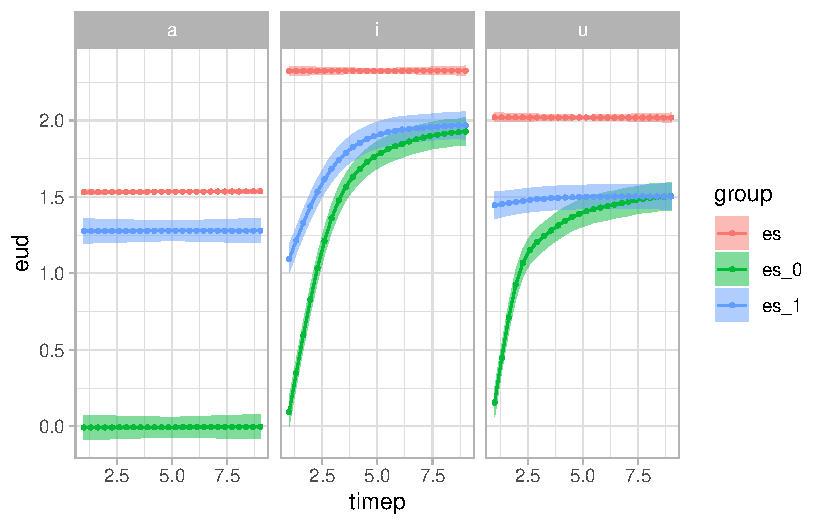
\includegraphics{manuscript_files/figure-pdf/fig-gam-3-1.pdf}

}

\caption{\label{fig-gam-3}Predicted Euclidean distance along the
duration of the vowel, for /a, i, u/ in simultaneous bilinguals (es),
beginners late bilinguals (es\_0) and advanced late bilinguals (es\_1)}

\end{figure}%

What follows is an example of how the model and results could be
reported in prose.

We fitted a Generalised Additive Model to Euclidean Distance values
taken along the duration of the vowels /a, i. u/ in simultaneous,
low-proficiency late and high-proficiency late English/Spanish
bilinguals. We included a parametric term for the variable
\texttt{group\_vowel} which is the combination of group (\texttt{es},
\texttt{es\_0}, \texttt{es\_1}) and vowel (\texttt{a}, \texttt{i},
\texttt{u}) to model mean differences in EUD between group/vowel, and a
smooth term over time point (\texttt{timep}) with \texttt{group\_vowel}
as a by-variable to model non-linear trajectories of EUD in each
group/vowel condition. We have also included a random factor smooth by
subject over time point to model by-subject differences in mean EUD and
trajectory shapes.

The simultaneous English/Spanish bilingual data (group \texttt{es}) in
Figure~\ref{fig-gam-3} clearly shows stable EUD throughout the duration
of vowels /a/, /i/ and /u/, indicating that no unstressed vowel
reduction occurs (of course, since the data is simulated, the EUD
trajectories are unnaturally flat). Moreover, the EUDs for each vowel
differ thus indicating that each vowel is distinguished despite absence
of stress as we would expect in Spanish. When looking at the beginner
late bilinguals (group \texttt{es\_0}), the plot indicates that /a/ is
reduced to {[}ə{]} (the EUD is 0), that /i/ and /u/ are strongly
diphthongised, and that the first part of the diphthong is close to
{[}ə{]} while the second part does not quite reach the EUD values of the
simultaneous English/Spanish bilinguals, again as we would expect in
English speakers learning Spanish.

In the high-proficiency late English/Spanish bilinguals we can observe
almost no reduction in /a/ (the EUD values are close to the simultaneous
bilinguals' values and flat) and a lesser degree of reduction in /i/ and
/u/, although the EUD value for the second part of the diphthongised
vowels still don't quite reach the value of the simultaneous bilinguals.
Moreover, the second part of /i/ and /u/ is very similar in both late
bilingual groups, thus suggesting that while there is less
diphthongisation in the high-proficiency group, this group still hasn't
developed simultaneous bilingual-like targets.

\section{Summary}\label{summary}

This introductory tutorial covered the basics of fitting non-linear
effects using Generalised Additive Models (GAMs) and the mixed-effects
counterpart Generalised Additive Mixed Models (GAMMs) with the mgcv and
tidygam packages in R.

Two literature-based simulated case studies were employed to illustrate
how to fit and plot GAMs. Case study 1 was about U-shaped learning and
focused on modelling non-linear effects with smooths (\texttt{s()} terms
in R syntax) and on obtaining model predictions for plotting. Case study
2 illustrated a time-series analysis of euclidean distance trajectories
of three vowels (/a, i, u/) of three bilingual groups (simultaneous
English/Spanish, low-proficiency late, high proficiency late). This case
study introduced readers to \texttt{by}- variables, used to model
effects of categorical factors on smooths, including interactions
between factors, and random factor smooth interactions, which fit random
effects.

This tutorial on its own will not be sufficient to develop an adequate
GAM analysis but constitutes a low barrier-to-entry for readers who are
interested in learning about GAMs. We encourage those who wish to run a
full GAM analysis to peruse the tutorials mentioned in the introduction:
Sóskuthy (2017), Sóskuthy (2021), Pedersen et al. (2019), Tamminga et
al. (2016), and Wieling (2018). Important topics that were not covered
here are: selection of type and number of basis functions in smooths,
autocorrelation and autoregressive models, statistical inference and
modelling other distribution families.

\section{Data availability statement}\label{data-availability-statement}

The compendium with code and data used in this tutorial can be found at
\url{https://github.com/stefanocoretta/gamm_biling}.

\newpage{}

\subsection*{References}\label{references}
\addcontentsline{toc}{subsection}{References}

\phantomsection\label{refs}
\begin{CSLReferences}{1}{0}
\bibitem[\citeproctext]{ref-aldrich2014acquisition}
Aldrich, A. C. (2014). \emph{Acquisition of {L}2 phonology: An acoustic
analysis of the centralization of {L}2 {S}panish /a/ in adult {L}1
{E}nglish-speaking learners}. MA Thesis. Brigham Young University.

\bibitem[\citeproctext]{ref-Amengual2020}
Amengual, M., \& Simonet, M. (2020). Language dominance does not always
predict cross-linguistic interactions in bilingual speech production.
\emph{Linguistic Approaches to Bilingualism}, \emph{10}(6), 847--872.
\url{https://doi.org/10.1075/lab.18042.ame}

\bibitem[\citeproctext]{ref-bland2016speech}
Bland, J. (2016). \emph{Speech style, syllable stress, and the
second-language acquisition of {S}panish /e/ and /o/}. MA thesis,
Virginia Polytechnic Institute; State University.

\bibitem[\citeproctext]{ref-Botezatu2024}
Botezatu, M. R., Misra, M., \& Kroll, J. F. (2024). Proficiency in a
second language influences processing of print-to-sound mappings.
\emph{Linguistic Approaches to Bilingualism}, \emph{14}(3), 285--309.
\url{https://doi.org/10.1075/lab.21063.bot}

\bibitem[\citeproctext]{ref-carlucci2013necessity}
Carlucci, L., \& Case, J. (2013). On the necessity of {U}-shaped
learning. \emph{Topics in Cognitive Science}, \emph{5}(1), 56--88.
\url{https://doi.org/10.1111/tops.12002}

\bibitem[\citeproctext]{ref-casani2020valutare}
Casani, E. (2020). Valutare la competenza morfosintattica in italiano
{L}2. Una validazione corpus-based dei livelli del {QCER}. In E. Nuzzo,
E. Santoro, \& I. Vedder (Eds.), \emph{Valutazione e misurazione delle
produzioni orali e scritte in italiano lingua seconda} (pp. 15--26).
Florence: Franco Cesati Editore.

\bibitem[\citeproctext]{ref-cazden1968acquisition}
Cazden, C. B. (1968). The acquisition of noun and verb inflections.
\emph{Child Development}, \emph{39}(2), 433--448.
\url{https://doi.org/10.2307/1126956}

\bibitem[\citeproctext]{ref-cobb2009pronunciacion}
Cobb, K. (2009). \emph{La pronunciaci{ó}n de vocales {á}tonas en
espa{ñ}ol: La aplicaci{ó}n de reglas fonol{ó}gicas por parte de
hablantes no-nativos del espa{ñ}ol}. MA Thesis. The University of
Arizona.

\bibitem[\citeproctext]{ref-cobb2015adult}
Cobb, K., \& Simonet, M. (2015). Adult second language learning of
{S}panish vowels. \emph{Hispania}, \emph{98}(1), 47--60.
\url{https://doi.org/10.1353/hpn.2015.0026}

\bibitem[\citeproctext]{ref-coretta2023}
Coretta, S. (2023). \emph{Tidygam: Tidy prediction and plotting of
generalised additive models}.
\url{/url\%7Bhttps://CRAN.R-project.org/package=tidygam\%7D}

\bibitem[\citeproctext]{ref-FuenteIglesias2022}
de la Fuente Iglesias, M., \& P'erez Castillejo, S. (2022). L1 phonetic
permeability and phonetic path towards a potential merger: The case of
galician mid vowels in bilingual production. \emph{Linguistic Approaches
to Bilingualism}, \emph{12}(2), 191--219.
\url{https://doi.org/10.1075/lab.19094.del}

\bibitem[\citeproctext]{ref-ervin_miller1963}
Ervin, S. M., \& Miller, W. R. (1963). Language development. In H. W.
Stevenson, J. C. Kagan, C. C. Spiker, N. B. Henry, \& H. G. Richey
(Eds.), \emph{Child psychology: The sixty-second yearbook of the
{National Society for the Study of Education}, {P}art 1} (pp. 108--143).
University of Chicago Press.

\bibitem[\citeproctext]{ref-gass_selinker_2008}
Gass, S., \& Selinker, L. (2008). \emph{Second language acquisition. An
introductory course}. New York: Routledge.

\bibitem[\citeproctext]{ref-geeslin2006longitudinal}
Geeslin, K. L., \& Guijarro-Fuentes, P. (2006). A longitudinal study of
copula choice: Following development in variable structures. In N.
Sagarra \& A. J. Toribio (Eds.), \emph{Selected procedures of the 9th
hispanic linguistics symposium} (pp. 144--156). Somerville, MA:
Cascadilla Proceedings Project.

\bibitem[\citeproctext]{ref-gigerenzer2004}
Gigerenzer, G. (2004). Mindless statistics. \emph{The Journal of
Socio-Economics}, \emph{33}(5), 587--606.
\url{https://doi.org/10.1016/j.socec.2004.09.033}

\bibitem[\citeproctext]{ref-hastie1986}
Hastie, T., \& Tibshirani, R. (1986). Generalized additive models.
\emph{Statistical Science}, \emph{1}(3), 297--310.
\url{https://doi.org/10.1201/9780203753781-6}

\bibitem[\citeproctext]{ref-iruela1997adquisicion}
Iruela, A. (1997). Adquisici{ó}n del vocalismo espa{ñ}ol por holandeses:
An{á}lisis en estilo semiespont{á}neo. \emph{Estudios de Fon{é}tica
Experimental IX}, 135--180.

\bibitem[\citeproctext]{ref-kellerman1985if}
Kellerman, E. (1985). If at first you do succeed... In S. M. Gass \& C.
G. Madden (Eds.), \emph{Input in {Second Language Acquisition}} (pp.
345--353). Rowley: Newbury.

\bibitem[\citeproctext]{ref-lightbown1983exploring}
Lightbown, P. (1983). Exploring relationships between developmental and
instructional sequences in {L}2 acquisition. In H. Seliger \& M. Long
(Eds.), \emph{Classroom oriented research in second language
acquisition} (pp. 217--243). Rowley, MA: Newbury House.

\bibitem[\citeproctext]{ref-long1990least}
Long, M. H. (1990). The least a second language acquisition theory needs
to explain. \emph{TESOL Quarterly}, \emph{24}(4), 649--666.
\url{https://doi.org/10.2307/3587113}

\bibitem[\citeproctext]{ref-luedecke2018}
Lüdecke, D. (2018). Ggeffects: Tidy data frames of marginal effects from
regression models. \emph{Journal of Open Source Software}, \emph{3}(26),
772. \url{https://doi.org/10.21105/joss.00772}

\bibitem[\citeproctext]{ref-marcus1992overregularization}
Marcus, G. F., Pinker, S., Ullman, M., Hollander, M., Rosen, T. J., Xu,
F., \& Clahsen, H. (1992). Overregularization in language acquisition.
\emph{Monographs of the Society for Research in Child Development},
\emph{57}(4), i--178. \url{https://doi.org/10.2307/1166115}

\bibitem[\citeproctext]{ref-martinez_celdran_1984}
Martínez Celdrán, E. (1984). \emph{Fon{é}tica}. Barcelona: Teide.

\bibitem[\citeproctext]{ref-mcelreath2019}
McElreath, R. (2019). \emph{Statistical rethinking: A {B}ayesian course
with examples in {R} and {S}tan}. Boca Raton, FL: CRC Press.

\bibitem[\citeproctext]{ref-pearl2010introduction}
Pearl, J. (2010). An introduction to causal inference. \emph{The
International Journal of Biostatistics}, \emph{6}(2).
\url{https://doi.org/10.2202/1557-4679.1203}

\bibitem[\citeproctext]{ref-pedersen2019}
Pedersen, E. J., Miller, D. L., Simpson, G. L., \& Ross, N. (2019).
Hierarchical generalized additive models in ecology: An introduction
with mgcv. \emph{PeerJ}, \emph{7}, e6876.
\url{https://doi.org/10.7717/peerj.6876}

\bibitem[\citeproctext]{ref-pliatsikas2013processing}
Pliatsikas, C., \& Marinis, T. (2013). Processing empty categories in a
second language: When naturalistic exposure fills the (intermediate)
gap. \emph{Bilingualism: Language and Cognition}, \emph{16}(1),
167--182. \url{https://doi.org/10.1017/S136672891200017X}

\bibitem[\citeproctext]{ref-rct2023}
R Core Team. (2023). \emph{R: A language and environment for statistical
computing}. R Foundation for Statistical Computing.
\url{https://www.R-project.org/}

\bibitem[\citeproctext]{ref-rumelhart2014learning}
Rumelhart, D. E., \& McClelland, J. L. (1986). On learning the past
tenses of {E}nglish verbs. Implicit rules or parallel distributed
processing? In J. L. McClelland \& D. E. Rumelhart (Eds.),
\emph{Parallel distributed processing: Explorations in the
microstructure of cognition}. Cambridge: MIT Press.

\bibitem[\citeproctext]{ref-shirai1990u}
Shirai, Y. (1990). {U}-shaped behavior in {L2} acquisition.
\emph{Variability in Second Language Acquisition: Proceedings of the
Tenth Meeting of the {Second Language Research Forum}}, \emph{2},
685--700.

\bibitem[\citeproctext]{ref-simpson2023}
Simpson, G. (2023). \emph{What do p-values mean in generalized additive
model?} Cross Validated.

\bibitem[\citeproctext]{ref-soskuthy2017}
Sóskuthy, M. (2017). \emph{Generalised additive mixed models for dynamic
analysis in linguistics: A practical introduction}. {a}rXiv.org
preprint, arXiv:1703.05339.

\bibitem[\citeproctext]{ref-soskuthy2021}
Sóskuthy, M. (2021). Evaluating generalised additive mixed modelling
strategies for dynamic speech analysis. \emph{Journal of Phonetics},
\emph{84}, 101017. \url{https://doi.org/10.1016/j.wocn.2020.101017}

\bibitem[\citeproctext]{ref-tamminga2016}
Tamminga, M., Ahern, C., \& Ecay, A. (2016). Generalized additive mixed
models for intraspeaker variation. \emph{Linguistics Vanguard},
\emph{2}(s1), 33--41. \url{https://doi.org/10.1515/lingvan-2016-0030}

\bibitem[\citeproctext]{ref-wieling2018}
Wieling, M. (2018). Analyzing dynamic phonetic data using generalized
additive mixed modeling: A tutorial focusing on articulatory differences
between {L}1 and {L}2 speakers of {E}nglish. \emph{Journal of
Phonetics}, \emph{70}, 86--116.
\url{https://doi.org/10.1016/j.wocn.2018.03.002}

\bibitem[\citeproctext]{ref-williams2022u}
Williams, S., Guijarro-Fuentes, P., \& Vulchanova, M. (2022). {U}-shaped
trajectories in an {L}2 context: Evidence from the acquisition of verb
morphology. \emph{Vigo International Journal of Applied Linguistics},
\emph{19}, 223--266. \url{https://doi.org/10.35869/vial.v0i19.3764}

\bibitem[\citeproctext]{ref-winter2013}
Winter, B. (2013). \emph{Linear models and linear mixed effects models
in {R} with linguistic applications}. {a}rXiv:1308.5499.
\url{/url\%7Bhttps://arxiv.org/abs/1308.5499\%7D}

\bibitem[\citeproctext]{ref-winter2020}
Winter, B. (2020). \emph{Statistics for linguists: An introduction using
{R}}. Routledge.

\bibitem[\citeproctext]{ref-wood2006}
Wood, S. (2006). \emph{Generalized additive models: An introduction with
{R}}. CRC Press.

\bibitem[\citeproctext]{ref-wood2011}
Wood, S. (2011). Fast stable restricted maximum likelihood and marginal
likelihood estimation of semiparametric generalized linear models.
\emph{Journal of the Royal Statistical Society (B)}, \emph{73}(1),
3--36.

\end{CSLReferences}




\end{document}
